\section{PLANNING \& CONTROL}

In this section, we present investigations on relevant techniques reported in
the literature for the decision-making system of self-driving cars, comprising
the route planning, behavior selection, motion planning, and control subsystems.

Towards the end, we also discuss the execution competency of an autonomous
system, also often referred to as motion control, is the process of converting
intentions into actions; its main purpose is to execute the planned intentions
by providing necessary inputs to the hardware level that will generate the
desired motions. Controllers map the interaction in the real world in terms of
forces, and energy, while the cognitive navigation and planning algorithms in an
autonomous system are usually concerned with the velocity and position of the
vehicle with respect to its environment. Measurements inside the control system
can be used to determine how well the system is behaving, and therefore the
controller can react to reject disturbances and alter the dynamics of the system
to the desired state. Models of the system can be used to describe the desired
motion in greater detail, which is essential for satisfactory motion execution.

\begin{figure}[h]
    \centering
    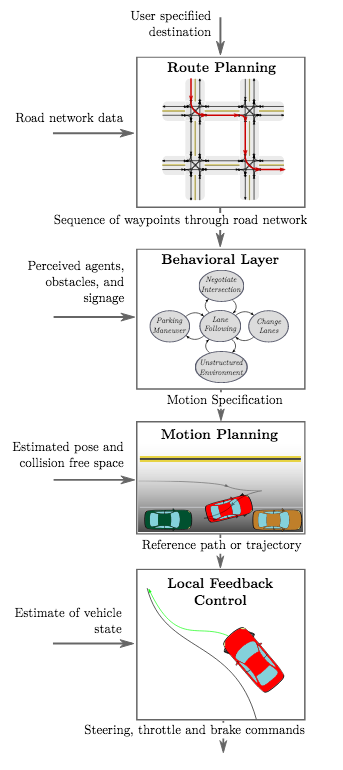
\includegraphics[height=0.9\textheight]{decision.png}
    \caption{Illustration  of  the  hierarchy  of  decision-making processes.  A  destination  is  passed  to  a  route  planner  that generates  a  route  through  the  road  network.  A  behavioral layer  reasons  about  the  environment  and  generates  a  motion specification  to  progress  along  the  selected  route.  A  motion planner  then  solves  for  a  feasible  motion  accomplishing  the specification. A feedback control adjusts actuation variables to correct errors in executing the reference path. }
    \label{fig:lidar}
\end{figure}

\subsection{Route Planning}

The route planning subsystem is responsible for computing a route through the
road network from the self-driving car’s initial position to the final position
defined by a user operator. If the road network is represented by a weighted
directed graph, whose edge weights denote the cost of traversing a road segment,
then the problem of computing a route can be reduced to the problem of finding
the shortest path in a weighted directed graph. However, for large road
networks, complexity times of classical shortest path algorithms, such as
Dijkstra and A*, are impractical.

In the last decade, there have been significant advances in the performance of
algorithms for route planning in road networks. Newly developed algorithms can
compute driving directions in milliseconds or less, even at continental scales.

Methods for route planning in road networks provide different trade-offs in
terms of query time, preprocessing time, space usage, and robustness to input
changes, among other factors. They can be mainly categorized into four classes
: goal-directed, separator-based, hierarchical, bounded-hop, and
combinations.

\subsection{Motion Planning}

When the behavioral layer decides on the driving behavior to  be  performed  in
the  current  context,  which  could  be,e.g.,  cruise-in-lane,  change-lane,
or  turn-right,  the  selected behavior  has  to  be  translated  into  a  path
or  trajectory  that can  be  tracked  by  the  low-level  feedback  controller.
The resulting  path  or  trajectory  must  be  dynamically  feasible  for the
vehicle, comfortable for the passenger, and avoid collisions with  obstacles
detected  by  the  on-board  sensors.  The  task  of finding  such  a  path  or
trajectory  is  a  responsibility  of  the motion planning system.

The  task  of motion  planning  for  an  autonomous  vehicle corresponds to
solving the standard motion planning problem as  discussed  in  the  robotics
literature. Exact  solutions  to  the motion  planning  problem  are  in  most
cases computationally intractable.  Thus,  numerical  approximation  methods
are typically  used  in  practice.  Among  the  most  popular  numerical
approaches are  variational  methods  that  pose  the  problem  as non-linear
optimization in a function space, graph-search approaches that construct
graphical discretization of the vehicle’s state space and search for a shortest
path using graph search methods,  and  incremental  tree-based  approaches  that
incrementally  construct  a  tree  of  reachable  states  from  the initial
state of the vehicle and then select the best branch of such a tree.

\subsubsection{Lane Graphs}

When the path planning problem involves driving on a structured road network, a
sufficient graph discretization may consist of edges representing the path that
the car should follow within each lane and paths that traverse intersections.
Road lane graphs are often partly algorithmically generated from higher-level
street network maps and partly human edited. An example of such a graph is in
Figure

\begin{figure}[H]
    \centering
    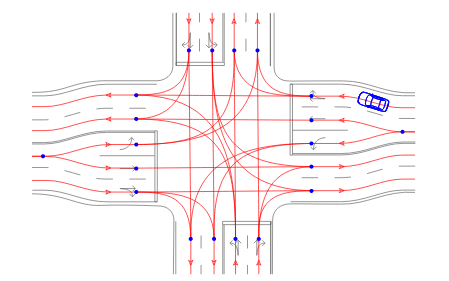
\includegraphics[width=0.9\textwidth]{handcraft.png}
    \caption{Hand-crafted  graph  representing  desired driving paths under normal circumstances.}
    \label{fig:handcraft}
\end{figure}


Although most of the time it is sufficient for the autonomous vehicle to follow
the paths encoded in the road lane graph, occasionally it must be able to
navigate around obstacles that were not considered when the road network graph
was de- signed or in environments not covered by the graph. Consider for example
a faulty vehicle blocking the lane that the vehicle plans to traverse – in such
a situation a more general motion planning approach must be used to find a
collision-free path around the detected obstacle.

\subsection{Trajectory Planning}

Trajectory planning involves generating a sequence of states from the
self-driving car’s current state to the next goal state, which specifies the
evolution of car’s states through time. Methods for trajectory planning can be
mainly categorized into four classes: graph search based, sampling based,
interpolating curve based, and numerical optimization based.

\subsubsection{Graph Search Based Techniques}
Graph search based techniques for trajectory planning extend those for path
planning in order to specify the evolution of car’s states over time. The most
common graph search based trajectory planning techniques of self-driving cars
are state lattice, elastic-band (EB), and A*.

\subsubsection{Sampling Based Techniques}
Sampling based techniques randomly sample the state space looking for a
connection between the car’s current state and the next goal state. The most
usual sampling based techniques for trajectory planning of self-driving cars are
rapidly- exploring random tree (RRT).

\subsubsection{Interpolating Curve Based Techniques}
Interpolating curve based techniques interpolate a previously known set of
points (e.g., road-map way points) and build a smoother trajectory that considers
car’s kinematic and dynamic constraints, comfort, obstacles, among other
parameters. The most common interpolating curve based techniques for trajectory
planning of self-driving cars are clothoid curves.

\subsubsection{Numerical Optimization}
Numerical optimization based techniques minimize or maximize a function with
constrained variables. The most common numerical optimization based techniques
for trajectory planning of self-driving cars are function optimization and
model-predictive methods.

\subsection{Control}

In the field of self-driving cars, control refers to the theory behind automatic
control of the engineering area, which covers the application of mechanisms to
operate and regulate processes without continuous direct human intervention. In
the simplest type of automatic control, a control subsystem compares the
process’s output with a desired input and uses the error (difference between the
process’s output and the desired input) to change the process’s input, such that
the process stays at its set point despite disturbances. In autonomous vehicles,
the automatic control theory is generally applied to path tracking and hardware
actuation methods. The role of a path tracking method is to stabilize the
execution of the motion plan in the presence of inaccuracies in the car’s model,
among others. The role of the hardware actuation control is to compute steering,
throttle and brake actuator inputs that execute the motion plan in the presence
of inaccuracies in actuators’ models and others.

Path tracking methods are also referred to as control techniques, because they
employ the automatic control theory and consider the path as the signal to be
controlled. However, in the area of autonomous vehicles, it is more appropriate
to refer to them as path tracking methods, in order to discern them from
hardware actuation control methods. Both of them are detailed in the next
subsections.

\subsubsection{Path Tracking Models}

Path tracking methods stabilize (i.e., reduce the error in) the execution of the
motion plan computed by the motion planning subsystem, in order to reduce
inaccuracies caused mainly by car’s motion model. They can be considered
simplified trajectory planning techniques, although they do not deal with
obstacles. The pure pursuit method is broadly used in self-driving cars for path
tracking, because of its simple implementation. It consists of finding a point
in the path at some look-ahead distance from the current path and turning the
front wheel so that a circular arc connects the center of the rear axle with the
point in the path, as shown in Figure \ref{fig:controlGeometry}. Thrun et al.
\cite{THR07} presents the control approach of the autonomous vehicle Stanley,
which consists of taking the front wheel position as the regulated variable.
Stanley’s control subsystem was able to drive the car at up to 60 km/h.

\begin{figure}[H]
    \centering
    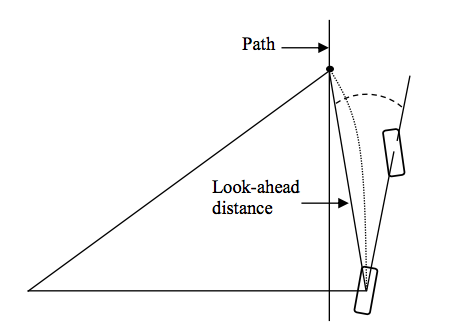
\includegraphics[width=0.5\textwidth]{controlGeometry.png}
    \caption{Pure Pursuit approach geometry.}
    \label{fig:controlGeometry}
\end{figure}

The Model Predictive Control (MPC) method is widely employed in driverless cars.
It consists of selecting control command inputs that will lead to desired
hardware outputs, using the car’s motion model to simulate and optimize outputs
over a prediction horizon in the future. Koga et al. \cite{KOG13} use the MPC
method for path tracking of a small electrical car. They employ the standard
bicycle model to predict car’s motion. The electrical car’s control subsystem
was able to drive the car at up to 20 km/h. Kritayakirana and Gerdes \cite{KRI12}
present the control approach of an Audi TTS, in which a dynamic motion model of
the car is used to enable path tracking at the limits of
handling. The car’s dynamic motion model considers the deviation from the path
plan due to tire slippage. Experimental results demonstrated that the Audi TTS
could achieve a speed of up to 160 km/h.

\subsubsection{Hardware Actuation Control Methods}

Hardware actuation control methods compute inputs for the steering, throttle,
and brake actuators of the car, which execute the motion plan computed by the
motion planning subsystem and mitigate inaccuracies caused primarily by
actuators’ models. One of the most common hardware actuation control methods for
self-driving cars is the feedback control. It involves applying a control
command input, observing the hardware output, and adjusting future inputs to
correct errors in actuators’ models. Hardware structures of the Audi TTS were
designed to achieve hard real-time control at 200 Hz. This high-speed hardware
enabled their control subsystem to drive the car at up to 160 km/h. Ziegler et
al. \cite{ZIE14a} employed a feedback control method for the control subsystem
of “Bertha”, which drove autonomously on the historic Bertha-
Benz-Memorial-Route in Germany. Bertha’s control subsystem was able to drive the
car at up to 100 km/h through the 103 km long Bertha-Benz-Memorial-Route. Li et
al. \cite{LI17} adopted the same control method in a Toyota Land Cruiser, which
was able to drive the car at up to 25 km/h.

Another popular hardware actuation method for autonomous vehicles is the
Proportional Integral Derivative (PID). It involves specifying a desired
hardware input and an error measure that accounts for how far the hardware
output is from the desired hardware input. In possession of this
information, a PID control method computes the hardware input, which is $K_p$
times the error measure (proportional to the error according to $K_d$), plus $K_i$
times the integral of the error, plus $K_d$ times the derivative of the error,
where $K_p, K_d$ and $K_i$ are parameters of the PID control method. Similar to
the feedback control technique, the PID control method can deal with the current
error, besides the accumulated past errors over time and future errors.
Zhao et al. \cite{ZHA12} used an adaptive PID method based on the generalized minimum
variance technique to implement the control subsystem of the driverless car
``Intelligent Pionner". Intelligent Pionner’s control subsystem was able to drive
the car at up to 60 km/h. Levinson et al. employed a mixture of a MPC
method, based on well-known physically based car models, and a feedforward PID
control technique for the control subsystem of the robotic car “Junior” \cite{MON08}
(Stanford University’s car that finished in second place in the 2007 DARPA Urban
Challenge). Junior’s control subsystem was able to drive the car at up to 56
km/h.